%!TEX root = ../../main.tex
\section{Metoder}

I dette projekt er der blevet brugt følgende arbejdsmetoder:
\begin{itemize}
	\item V-Modellen
	\item SCRUM
	
\end{itemize}

\subsection{V-Modellen}

V-Modellen, som er en udviklingsmodel, er blevet brugt til at lave løbende test i dette projekt. Da der laves test sideløbende sikres der, at systemet virker efter hensigten. På figur \ref{VModel} kan V-Modellen ses.

\begin{figure}[H]
	\centering
	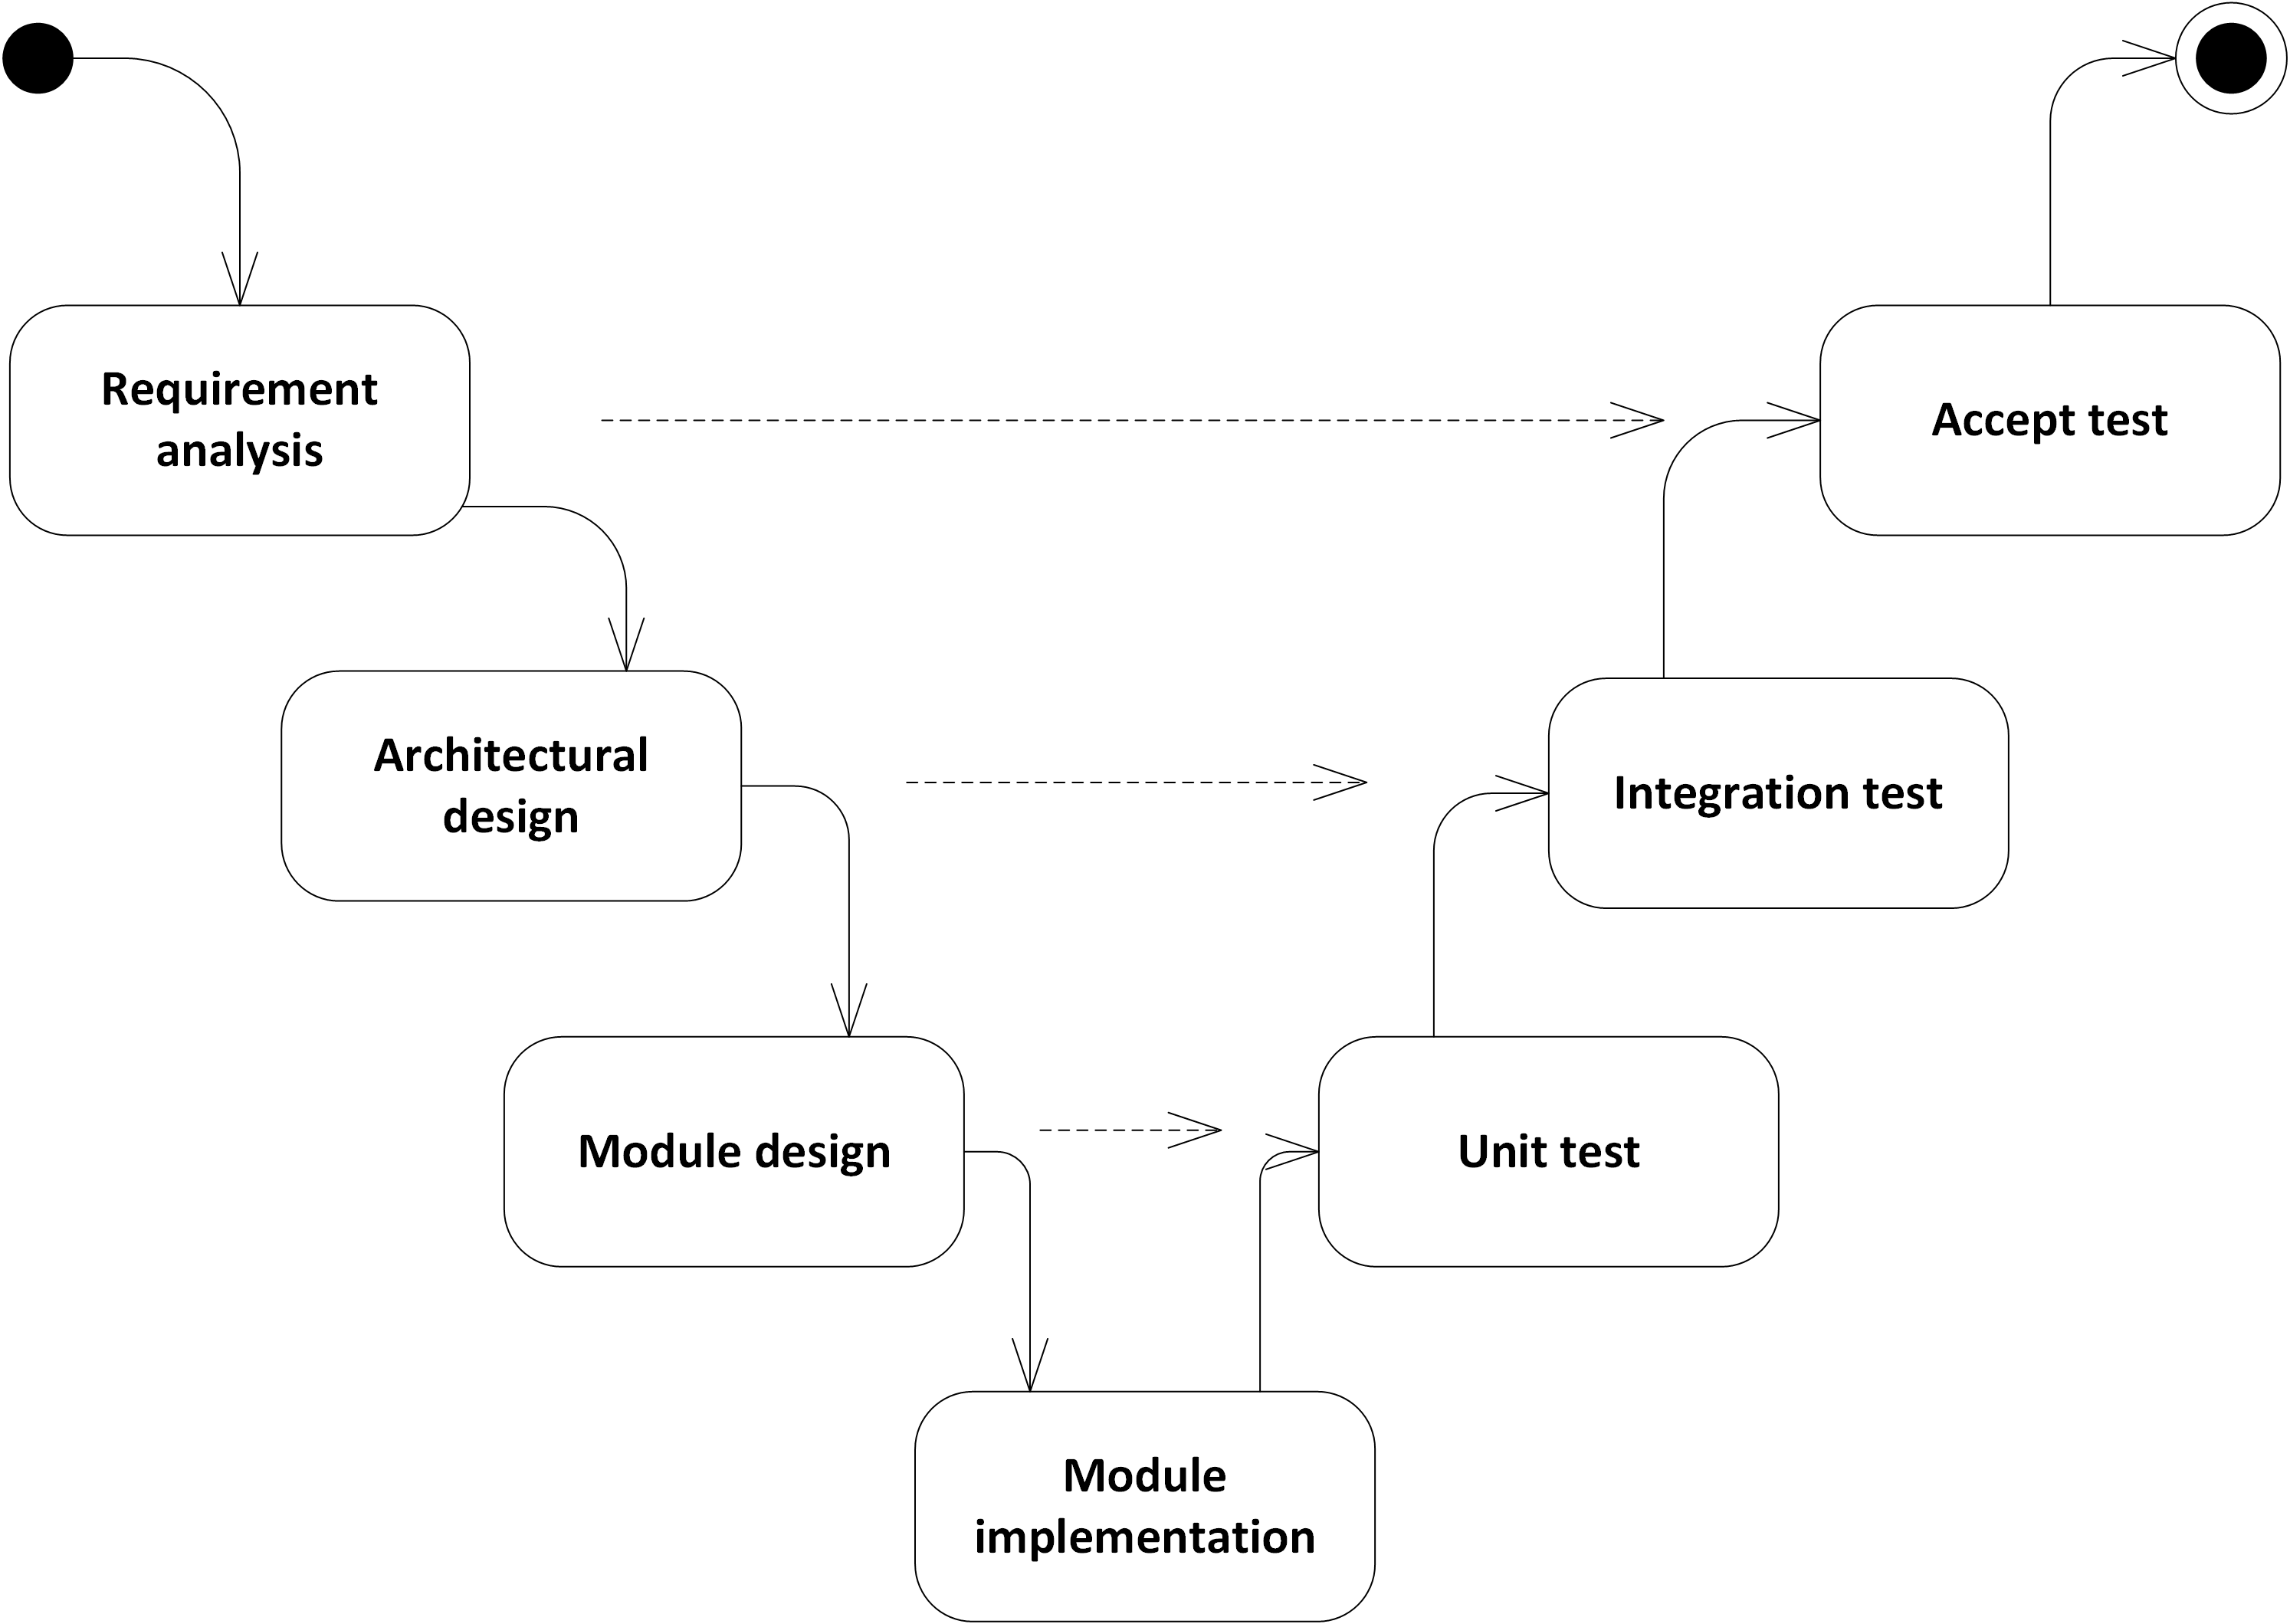
\includegraphics[scale=1.0]{Rapport/VModel.PNG}
	\caption{V-Modellen}
	\label{VModel}
\end{figure} 
Den første udviklingsfase er udarbejdelse af kravspecifikationen. Her udvikles der en tilhørende accepttest, der verificerer systemets overordnede funktionalitet. Den næste fase er systemarkitekturen.
I denne fase udvikles test af integrationen mellem implementerede moduler. Under design og implementering som udgør den sidste fase i udviklingen, udføres der løbende unit test af de implementerede moduler.

\subsection{SCRUM}
Udviklingsmetoden har være Scrum inspireret, da processen ikke har været fuld ud tilrettelagt, er det ikke ren Scrum. En af grundene har været at processen bliver uforudsigelig, når der bruges nye værktøjer og derfor har der været behov for fleksible tidsplaner og hyppig gennemgange. 
\newline
\newline
I dette projekt er det blevet anvendt til at dele større opgaver op i små dele til de forskellige sprints, samt til at holde daglige møder om arbejdet og opgaverne. 


